% Prognosequalität 2025/26 -- Paper
% Bauen: latexmk prognoseguete-2025-26.tex   (schreibt build/prognoseguete-2025-26.pdf)
% Zahlen und Abbildungen: scripts/evaluate_forecast_quality.R, dann
% scripts/analyze_forecast_quality.R (siehe Anhang B).
\documentclass[11pt,a4paper,parskip=half,numbers=noenddot]{scrartcl}

\usepackage[ngerman]{babel}
\AtBeginDocument{\shorthandoff{"}}
\usepackage{fontspec}
\usepackage{unicode-math}
\setmainfont{Source Serif Pro}
\setsansfont{Inter}[Scale=MatchLowercase]
\setmonofont{Source Code Pro}[Scale=MatchLowercase]
\setmathfont{STIX Two Math}[Scale=MatchLowercase]

\usepackage{microtype}
\usepackage{csquotes}
\usepackage{xcolor}
\usepackage{booktabs,tabularx,array,multirow}
\usepackage{graphicx}
\usepackage{adjustbox}
\usepackage{amsmath,mathtools}
\usepackage{caption}
\usepackage[most]{tcolorbox}
\usepackage{enumitem}
\usepackage{scrlayer-scrpage}
\usepackage[locale=DE,group-minimum-digits=4,group-separator={\,}]{siunitx}
\usepackage{xurl}
\usepackage[hidelinks]{hyperref}

\definecolor{ink}{HTML}{15130F}
\definecolor{ink2}{HTML}{312E29}
\definecolor{ink3}{HTML}{6B655C}
\definecolor{surface2}{HTML}{F5F3EE}
\definecolor{akzent}{HTML}{B0261E}
\definecolor{ocker}{HTML}{B8893A}

\addtokomafont{disposition}{\rmfamily\mdseries\color{ink}}
\addtokomafont{section}{\Large}
\addtokomafont{subsection}{\large}
\addtokomafont{pageheadfoot}{\sffamily\footnotesize\color{ink3}}
\captionsetup{font={small},labelfont={sf,bf},labelsep=period}
\pagestyle{scrheadings}
\clearpairofpagestyles
\ohead{Prognosequalität 2025/26}
\ofoot*{\pagemark}
\setlist{itemsep=2pt,topsep=4pt}
\setlength{\emergencystretch}{2em}

\newtcolorbox{merke}[1][]{enhanced,breakable,colback=surface2,colframe=surface2,
  borderline west={3pt}{0pt}{ocker},arc=0pt,left=10pt,right=8pt,top=6pt,bottom=6pt,
  fonttitle=\sffamily\bfseries\small,coltitle=ink,title={#1},
  attach title to upper={\par\smallskip}}

\DeclareUrlCommand\datei{\def\UrlFont{\ttfamily\small}}
\newcommand{\code}[1]{\texttt{#1}}
\newcommand{\RPS}{\operatorname{RPS}}
\newcommand{\BS}{\operatorname{BS}}
\newcommand{\abb}[1]{Abbildung~\ref{#1}}
\newcommand{\tab}[1]{Tabelle~\ref{#1}}

\hypersetup{pdftitle={Wie gut waren die Prognosen? Saison 2025/26},pdfauthor={Christoph Schwerdtfeger}}

\begin{document}

\begin{flushleft}
  {\sffamily\small\color{ink3} 30 Punkte · fussball.csdatascience.de · Bericht vom 11.~Oktober 2026\par}
  \vspace{4pt}
  {\color{akzent}\rule{40pt}{2pt}\par}
  \vspace{10pt}
  {\fontsize{24}{28}\selectfont Wie gut waren die Prognosen?\par}
  \vspace{6pt}
  {\large\color{ink2} Eine Evaluation des League Simulators für Bundesliga,
  2.~Bundesliga und 3.~Liga in der Saison 2025/26\par}
  \vspace{8pt}
  {\sffamily\small Christoph Schwerdtfeger\par}
\end{flushleft}

\begin{abstract}
\noindent
Der League Simulator schätzt mit ELO-Werten, einem Poisson-Tormodell und
\num{10000} Monte-Carlo-Durchläufen, mit welcher Wahrscheinlichkeit jede
Mannschaft auf jedem Tabellenplatz landet. Wir rechnen diese Prognose für die
Saison 2025/26 vor jedem Spieltag nach, für drei Ligen also 106-mal, und
messen sie an den Endtabellen. Dazu dienen der Ranked Probability Score, der
Brier-Score, der logarithmische Score, Brier-Scores für Meisterschaft, Auf-
und Abstieg sowie Kalibrierungsdiagramme. Als naive Vergleichsprognosen
dienen die jeweils aktuelle Tabelle und vor Saisonbeginn die Tabelle der
Vorsaison. Über die Saison gemittelt ist das Modell in allen drei Ligen klar
besser als die aktuelle Tabelle. Der Ranked Probability Score sinkt um
35 bis 44~Prozent, und an 104 der 106 Spieltage liegt das Modell vorn. Als
reine Rangfolge ist der Vorsprung kleiner. In der zweiten Saisonhälfte der
3.~Liga ist die aktuelle Tabelle sogar gleichauf. Vor Saisonbeginn schlägt
das Modell die Vorsaisontabelle in jeder Liga deutlich. In der 2.~Bundesliga
und der 3.~Liga ist es dann aber kaum besser als eine Gleichverteilung,
nach dem logarithmischen Score sogar schlechter. Ursachen sind die
Überschätzung von Absteigern und eine zu große Schärfe bei mittleren und
hohen Wahrscheinlichkeiten. Die 1X2-Prognosen der Einzelspiele sind
brauchbar, unterschätzen aber den Heimvorteil der Saison 2025/26 um rund fünf
Prozentpunkte.
\end{abstract}

\section{Einleitung}

Seit 2015 veröffentlicht \emph{30 Punkte} für die Bundesliga nach jedem
Spieltag eine Wahrscheinlichkeitstabelle: Mit wie viel Prozent wird der FC
Bayern Meister, mit wie viel steigt der HSV ab? Heute läuft das Modell unter
dem Namen League Simulator für zehn Ligen und rechnet nach jedem Spiel neu.
Die Zahlen sind als Wahrscheinlichkeiten gemeint, nicht als Tipps. Ob sie
etwas taugen, zeigt sich deshalb nicht an einem einzelnen Ausgang. Es zeigt
sich erst, wenn man viele Prognosen mit dem vergleicht, was tatsächlich
eingetreten ist.

Eine erste solche Bilanz erschien am 15.~Mai 2016 für die Bundesliga
2015/16~\cite{30punkte2016}. Sie sammelte für jeden Club und jeden Platz die
Prognosen aller 33~Spieltage und stellte sie den Endplätzen gegenüber, in
einem Kalibrierungsdiagramm und in Verlaufskurven der Wahrscheinlichkeit für
den tatsächlichen Endplatz. Das Urteil lautete: \enquote{nicht allzu
schlecht}. Bis 10~Prozent unterschätzte das Modell die Häufigkeiten leicht,
oben war es \enquote{nicht mutig genug}, und von rund \num{2100} Prognosen
unter 2~Prozent traten 12 ein.

Dieser Bericht greift beide Darstellungen auf und ergänzt, was 2016 fehlte:
\begin{enumerate}
  \item \textbf{Übliche Gütemaße} für probabilistische Prognosen, also
        Ranked Probability Score, Brier-Score und logarithmischer Score, für
        die ganze Platzverteilung und für einzelne Ereignisse wie Meisterschaft
        oder Abstieg (Abschnitt~\ref{sec:masse}).
  \item \textbf{Naive Vergleichsprognosen.} Während der Saison ist das die
        jeweils aktuelle Tabelle, vor dem ersten Spieltag die Endtabelle der
        Vorsaison. Eine Prognose, die diese Maßstäbe nicht schlägt, braucht
        niemand.
  \item \textbf{Drei Ligen} statt einer: Bundesliga, 2.~Bundesliga und
        3.~Liga, zusammen 56~Mannschaften und 992~Spiele.
  \item \textbf{Die Einzelspiel-Prognosen} (Sieg, Remis, Niederlage), auf
        denen die Tabellenprognose aufbaut.
\end{enumerate}

\section{Das Modell in Kürze}\label{sec:modell}

Das Handbuch zum League Simulator beschreibt das Modell ausführlich, hier
genügt eine Skizze. ELO-Werte haben sich als Grundlage für
Fußballprognosen bewährt~\cite{hvattum2010}.

\paragraph{Stärke.} Jede Mannschaft trägt einen ELO-Wert $E$. Nach jedem
Spiel verschiebt sich die ELO beider Mannschaften um
$\delta = k\,m\,(S - p_h)$. Dabei ist $S \in \{0, \frac12, 1\}$ das Ergebnis
aus Sicht der Heimmannschaft und $p_h = 1/(1+10^{(E_a - E_h - H)/400})$ ihr
erwarteter Score. Es gilt $k = 20$, und $m = \sqrt{\max(|g_h - g_a|, 1)}$
gewichtet die Tordifferenz. Der Heimvorteil $H$ beträgt heute 40
ELO-Punkte. Während der Saison 2025/26 war produktiv noch $H = 65$
eingestellt (Abschnitt~\ref{sec:robust}).

\paragraph{Ergebnis.} Aus $\Delta = E_h + H - E_a$ folgen die
Torerwartungen $\lambda_{h,a} = \max(\pm s\,\Delta + c,\ 0{,}001)$ mit
$s = 0{,}0017855$ und $c = 1{,}32184$. Die Tore beider Mannschaften sind
unabhängig Poisson-verteilt. Daraus ergeben sich in geschlossener Form die
Wahrscheinlichkeiten für Heimsieg, Remis und Auswärtssieg, die
Abschnitt~\ref{sec:spiele} bewertet.

\paragraph{Tabelle.} Eine Iteration spielt die Saison vom ELO-Stand zum
Saisonstart durch. Gespielte Spiele gehen mit ihrem Ergebnis ein, offene
werden gezogen. Die ELO wird in beiden Fällen fortgeschrieben, ist also
innerhalb einer simulierten Saison dynamisch. Am Ende wird nach Punkten,
Tordifferenz und Toren sortiert. Aus \num{10000} Iterationen entsteht die
Matrix $P_{tp}$, die Wahrscheinlichkeit, dass Mannschaft $t$ auf Platz $p$
endet. Sie ist die Heatmap auf jeder Ligaseite.

\paragraph{Startwerte.} Die ELO zum Saisonstart ist die ELO am Ende der
Vorsaison, 1:1 übertragen, ohne Rückführung zur Mitte und unabhängig von
Auf- oder Abstieg. Mannschaften ohne beobachtete Vorsaison bekommen einen
Basiswert. In der 3.~Liga 2025/26 betraf das die vier Aufsteiger aus den
Regionalligen. Sie starteten alle mit $1\,064{,}08$, dem Mittel der vier
Absteiger der Vorsaison.

\section{Daten und Versuchsaufbau}\label{sec:aufbau}

\paragraph{Saison und Daten.} Ausgewertet wird die Saison 2025/26
(API-Football, Saison 2025). Das sind 306~Hauptrundenspiele in der Bundesliga
und der 2.~Bundesliga sowie 380 in der 3.~Liga, alle mit Status
\enquote{beendet}. Relegationsspiele zählen nicht zur Tabelle und bleiben
außen vor. Die Endtabelle wird aus den Ergebnissen nach Punkten, Tordifferenz
und Toren berechnet. Sie enthält keine vollständigen Gleichstände, ein
direkter Vergleich ist also nirgends nötig. Punktabzüge am grünen Tisch kennt
das Modell nicht. Für 2025/26 sind in den drei Ligen keine bekannt, mit den
amtlichen Tabellen abgeglichen wurde das aber nicht.

\paragraph{Ex ante.} Die Start-ELO stammen aus
\datei{RCode/TeamList_2025.csv}, im Repository seit dem 19.~Juli 2025, also
vor dem ersten Spieltag. Alles Weitere hängt nur an Ergebnissen, die zum
jeweiligen Zeitpunkt schon feststanden. Die Prognosen sind damit echte
Vorhersagen, keine Anpassung im Nachhinein.

\paragraph{Rückrechnung statt Archiv.} Die damals veröffentlichten Heatmaps
wurden nicht archiviert. Wir rechnen sie deshalb mit dem heutigen
Rust-Server nach. Für jeden Spieltag $t$ gilt als Stichtag der erste Anpfiff
von Spieltag $t$. Alle vorher beendeten Spiele gehen mit Ergebnis ein, der
Rest ist offen. So sieht die Prognose aus, die die Website am Vorabend des
Spieltags zeigte. Nachholspiele fließen ein, sobald sie gespielt sind. Das
ergibt 34~Prognosen für die Bundesliga und die 2.~Bundesliga und 38 für die
3.~Liga. Die Prognose \enquote{vor Spieltag~1} ist die Vorsaisonprognose. Jede
Prognose beruht auf \num{10000} Iterationen. Der Monte-Carlo-Fehler einer
einzelnen Wahrscheinlichkeit liegt damit unter 0,5~Prozentpunkten und ist
für alle folgenden Aussagen unerheblich.

\paragraph{Naive Vergleichsprognosen.}
\begin{description}[font=\sffamily\bfseries\small]
  \item[Aktuelle Tabelle] Der Platz zum Stichtag gilt als Prognose für den
        Endplatz. Gleichstände in Punkten, Tordifferenz und Toren entscheidet
        der Vorsaisonschlüssel. Vor Spieltag~1 ist die aktuelle Tabelle also
        die Vorsaisontabelle.
  \item[Vorsaison] Die Endtabelle der Vorsaison, auf die neue Liga
        übertragen. Oben stehen die Absteiger aus der höheren Liga, in deren
        Reihenfolge. Es folgen die verbliebenen Mannschaften nach ihrem
        Vorsaisonplatz und am Ende die Aufsteiger nach ihrem Platz in der
        tieferen Liga. Regionalliga-Meister verschiedener Staffeln werden
        nach Punkten je Spiel geordnet. Mit dieser Regel ist der Absteiger
        aus der Bundesliga der Favorit der 2.~Bundesliga, so wie ihn auch
        viele Saisonvorschauen sehen.
  \item[Gleichverteilung] Jeder Platz mit Wahrscheinlichkeit $1/n$. Sie
        dient als Nullpunkt: Wer sie nicht schlägt, weiß nichts.
  \item[Klimatologie] Für Ereignisse wie den Abstieg ist das der Anteil der
        Plätze, also zum Beispiel $2/18$. Für Einzelspiele sind es die
        Heim-, Remis- und Auswärtsquoten der Vorsaison in derselben Liga.
\end{description}
Die beiden Tabellenprognosen sind Punktprognosen. Für die
Wahrscheinlichkeitsmaße fassen wir sie als degenerierte Verteilung auf, mit
100~Prozent auf dem prognostizierten Platz. Das ist die übliche Lesart, aber
eine strenge: Eine Punktprognose kann für \enquote{knapp daneben} keine
Teilpunkte bekommen. Deshalb vergleichen wir zusätzlich Rangmaße, die beide
Prognosearten gleich behandeln.

\section{Gütemaße}\label{sec:masse}

Es seien $n$ die Zahl der Mannschaften, $P_{t1},\dots,P_{tn}$ die
Platzverteilung von Mannschaft $t$ und $r_t$ ihr tatsächlicher Endplatz. Alle
Maße werden je Mannschaft und Stichtag berechnet und dann gemittelt. Bei allen
gilt: kleiner ist besser.

\paragraph{Ranked Probability Score (RPS).} Das Hauptmaß dieses Berichts.
Er vergleicht kumulierte Verteilungen~\cite{epstein1969} und
belohnt deshalb Wahrscheinlichkeitsmasse \emph{nahe} am richtigen Platz:
\begin{equation}
  \RPS_t = \frac{1}{n-1} \sum_{k=1}^{n-1}
           \Bigl(\sum_{p \le k} P_{tp} - \mathbf{1}[r_t \le k]\Bigr)^2 .
\end{equation}
Für geordnete Ausgänge wie Tabellenplätze oder Sieg, Remis und Niederlage
ist er das übliche Maß~\cite{constantinou2012}. Eine Mannschaft, die mit
Sicherheit auf dem richtigen Platz erwartet wird, erhält 0. Die
Gleichverteilung erhält bei 18 Mannschaften im Mittel 0,176.

\paragraph{Brier-Score.} Die quadratische Abweichung über alle
Plätze~\cite{brier1950}, $\BS_t = \sum_p (P_{tp} - \mathbf{1}[p = r_t])^2$,
mit Werten zwischen 0 und 2. Er kennt keine Nähe: Platz 5 statt 4 kostet so
viel wie Platz 18 statt 4.

\paragraph{Logarithmischer Score.} $-\ln P_{t r_t}$, die
\enquote{Überraschung} über den tatsächlichen Ausgang. Er bestraft
Sicherheit, die sich als falsch erweist, beliebig hart. Monte-Carlo-Nullen
werden durch $1/(2N) = 0{,}00005$ ersetzt. Das war hier nie nötig: Kein
tatsächlicher Endplatz hatte je Wahrscheinlichkeit null. Für Punktprognosen
ist er unendlich und wird nur für das Modell berichtet.

Alle drei Maße sind \emph{strikt proper}~\cite{gneiting2007}. Wer seine
wahre Einschätzung meldet, schneidet im Erwartungswert am besten ab.

\paragraph{Ereignisse.} Für eine Platzgruppe $G$, etwa die Abstiegsplätze,
ist die Prognose $q_t = \sum_{p \in G} P_{tp}$ und der Brier-Score
$\frac1M\sum (q_t - o_t)^2$ mit $o_t = \mathbf 1[r_t \in G]$. Die
\emph{Skill Score} gegenüber einer Referenz ist $1 - \BS/\BS_{\text{ref}}$.
Sie ist positiv, wenn das Modell besser ist, und erreicht höchstens 1.

\paragraph{Rangmaße.} Als Punktprognose des Modells dient der erwartete
Platz $\bar p_t = \sum_p p\,P_{tp}$. Gemessen werden der mittlere absolute
Platzfehler $\frac1n\sum_t |\bar p_t - r_t|$ und Spearmans
Rangkorrelation zwischen prognostizierter und tatsächlicher Reihenfolge.

\paragraph{Kalibrierung.} Wie 2016 sammeln wir alle Einzelprognosen \enquote{Mannschaft $t$ landet auf Platz $p$} über alle Stichtage und Ligen, teilen sie
nach der prognostizierten Wahrscheinlichkeit in Klassen und vergleichen
jede Klasse mit der beobachteten Trefferquote. Bei guter Kalibrierung liegen
die Punkte auf der Diagonalen.

\begin{merke}[Zur Unabhängigkeit]
Die Prognosen eines Stichtags sind nicht unabhängig voneinander: Steht ein
Team sicher auf Platz~1, kann kein anderes dort stehen. Auch die Prognosen
aufeinanderfolgender Spieltage hängen stark zusammen. Die
\num{37232}~Einzelprognosen des Kalibrierungsdiagramms enthalten deshalb viel
weniger unabhängige Information, als ihre Zahl vermuten lässt. Wir geben
daher kaum formale Tests an. Die einzige Ausnahme ist ein Vorzeichentest
über Mannschaften (Abschnitt~\ref{sec:verlauf}).
\end{merke}

\section{Ergebnisse}

\subsection{Vor der Saison}\label{sec:vorsaison}

\begin{table}[!htbp]
\centering\footnotesize\setlength{\tabcolsep}{3.5pt}
\caption{Prognose vor Spieltag~1 gegen die Vorsaisontabelle. RPS, Brier und
Log: je Mannschaft gemittelt. Platzfehler: mittlerer absoluter Fehler,
Modell mit erwartetem Platz (in Klammern: mit ganzzahliger Rangfolge).
$\rho$: Spearman-Korrelation mit der Endtabelle.}\label{tab:vorsaison}
\begin{tabular}{@{}l rrr rrr r rr rr@{}}
\toprule
& \multicolumn{3}{c}{RPS} & \multicolumn{3}{c}{Brier} & \multicolumn{1}{c}{Log}
& \multicolumn{2}{c}{Platzfehler} & \multicolumn{2}{c}{$\rho$} \\
\cmidrule(lr){2-4}\cmidrule(lr){5-7}\cmidrule(lr){8-8}\cmidrule(lr){9-10}\cmidrule(l){11-12}
Liga & Mod. & Vors. & Gleich & Mod. & Vors. & Gleich & Mod.\,/\,Gleich & Mod. & Vors. & Mod. & Vors. \\
\midrule
Bundesliga    & \textbf{0,111} & 0,222 & 0,176 & \textbf{0,888} & 1,889 & 0,944 & 2,46\,/\,2,89 & \textbf{2,8} (3,1) & 3,8 & \textbf{0,73} & 0,64 \\
2. Bundesliga & \textbf{0,171} & 0,301 & 0,176 & 0,945 & 2,000 & 0,944 & 2,91\,/\,2,89 & \textbf{4,4} (5,0) & 5,1 & \textbf{0,27} & 0,25 \\
3. Liga       & 0,176 & 0,279 & \textbf{0,175} & \textbf{0,947} & 1,700 & 0,950 & 3,03\,/\,3,00 & \textbf{4,8} (5,6) & 5,3 & 0,14 & \textbf{0,18} \\
\bottomrule
\end{tabular}
\end{table}

\tab{tab:vorsaison} zeigt die Prognose vor dem ersten Spieltag. Nach RPS
und Brier schlägt das Modell die Vorsaisontabelle in allen drei Ligen
deutlich. Das liegt aber zum großen Teil an der Form der Prognose: Die
Vorsaisontabelle setzt alles auf einen Platz und bezahlt jeden Fehler voll.
Fairer ist der Vergleich der Rangmaße. Dort liegt das Modell in der
Bundesliga klar vorn (Platzfehler 2,8 gegen 3,8, $\rho = 0{,}73$ gegen
$0{,}64$). In der 2.~Bundesliga ist es knapp vorn, in der 3.~Liga
gleichauf.

Ernüchternd ist der Vergleich mit der Gleichverteilung. In der
2.~Bundesliga ist das Modell vor der Saison nur wenig besser als
\enquote{jeder Platz gleich wahrscheinlich}, in der 3.~Liga gleich gut. Nach
dem logarithmischen Score ist es in beiden Ligen sogar \emph{schlechter} als
die Gleichverteilung (2,91 gegen $\ln 18 = 2{,}89$, 3,03 gegen
$\ln 20 = 3{,}00$). Es hat also einigen Mannschaften Plätze fast
ausgeschlossen, auf denen sie dann landeten. In diesen beiden Ligen
erklärten Vorsaison-ELO und Vorsaisonplatz die Endtabelle 2025/26 kaum
($\rho \le 0{,}27$).

\paragraph{Woran es lag.} Die Mannschaftstabellen im Anhang~A zeigen ein
klares Muster. Alle vier Absteiger, die eine Liga tiefer neu ins Feld kamen,
setzte das Modell vor der Saison auf Rang~1, 2 oder~5:
\begin{itemize}
  \item Holstein Kiel (Modell 1., Ende 12.) und VfL Bochum (2., Ende 9.)
        in der 2.~Bundesliga,
  \item SSV Ulm (1., Ende 19.) und Jahn Regensburg (5., Ende 13.) in der
        3.~Liga.
\end{itemize}
Im Mittel landeten sie 6,6~Plätze schlechter als ihr erwarteter Platz. Bei
den verbliebenen Mannschaften liegt diese Verzerrung bei $+0{,}5$, bei den
Aufsteigern bei $+0{,}4$ Plätzen. Die ELO eines Absteigers stammt aus einer
stärkeren Liga und wird 1:1 übertragen, ohne Rückführung zur Mitte. Dass
ein Absteiger meist Stammspieler verliert und sich neu sortieren muss, kann
sie nicht wissen. Die Vorsaisontabelle macht denselben Fehler, nur stärker,
denn sie setzt die Absteiger ganz nach oben.

Die größten Ausreißer in die andere Richtung waren FC Schalke~04 und der
MSV Duisburg. Schalke war Vierzehnter der Vorsaison und hatte nur die
dreizehnthöchste Start-ELO der 2.~Bundesliga, wurde aber Meister. Das Modell
gab dafür vor der Saison 1,5~Prozent. Duisburg startete als
Regionalliga-Aufsteiger mit dem Basiswert und wurde Vierter. In der
Bundesliga lag das Modell dagegen oben richtig: Bayern Meister mit
48~Prozent (bester Wert der Liga), Dortmund, Leipzig und Stuttgart unter den
ersten sechs.

\subsection{Im Saisonverlauf}\label{sec:verlauf}

\begin{figure}[!htbp]
\centering
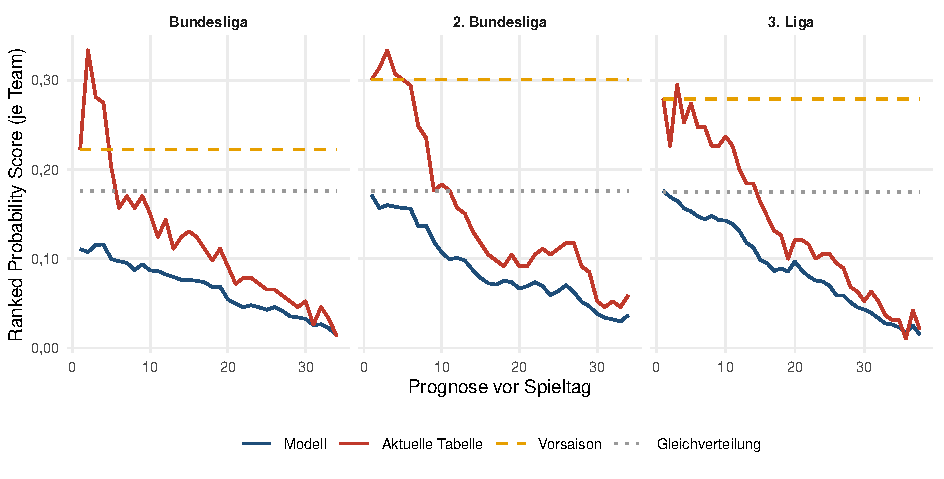
\includegraphics[width=\textwidth]{abbildungen/rps_verlauf.pdf}
\caption{Ranked Probability Score je Mannschaft, gemittelt über die Liga,
für die Prognose vor jedem Spieltag. Die Vorsaison ist als feste Prognose
eine Waagerechte.}\label{fig:rps}
\end{figure}

\abb{fig:rps} zeigt den RPS im Saisonverlauf. Das Modell (blau) liegt an
104 von 106~Stichtagen unter der aktuellen Tabelle (rot). Die beiden
Ausnahmen sind die Prognosen vor dem letzten Spieltag der Bundesliga und vor
dem 36.~Spieltag der 3.~Liga, an denen die Unterschiede verschwindend klein
sind. Der Abstand ist in den ersten zehn Spieltagen am größten. Hier
schwankt die Tabelle nach jedem Spieltag stark, während das Modell den
wenigen Ergebnissen nur so viel Gewicht gibt, wie sie verdienen. Schon nach
dem ersten Spieltag ist die aktuelle Tabelle in jeder Liga schlechter als
die Gleichverteilung (graue Linie). Darunter kommt sie erst mit der Prognose
vor dem 6.~Spieltag (Bundesliga), dem 12. (2.~Bundesliga) und dem 15.
(3.~Liga). Das Modell liegt in den beiden oberen Ligen von Anfang an
darunter, in der 3.~Liga ab dem zweiten Stichtag.

\begin{table}[!htbp]
\centering\footnotesize\setlength{\tabcolsep}{3.5pt}
\caption{Saisonmittel über alle Stichtage (jeder Spieltag gleich gewichtet).
RPSS: Skill Score des RPS gegenüber der aktuellen Tabelle. Hin/Rück: Mittel
über die erste bzw.\ zweite Hälfte der Stichtage.}\label{tab:saison}
\begin{adjustbox}{max width=\textwidth}
\begin{tabular}{@{}l rrr rr rr rr@{}}
\toprule
& \multicolumn{3}{c}{RPS} & \multicolumn{2}{c}{Brier} & \multicolumn{2}{c}{Platzfehler} & \multicolumn{2}{c}{$\rho$} \\
\cmidrule(lr){2-4}\cmidrule(lr){5-6}\cmidrule(lr){7-8}\cmidrule(l){9-10}
Liga & Modell & Tabelle & RPSS & Modell & Tabelle & Modell & Tabelle & Modell & Tabelle \\
\midrule
Bundesliga    & \textbf{0,066} & 0,119 & 44\,\% & \textbf{0,78} & 1,40 & \textbf{1,71} & 2,02 & \textbf{0,88} & 0,81 \\
\quad Hin\,/\,Rück & 0,092\,/\,0,041 & 0,176\,/\,0,062 & & & & 2,38\,/\,1,04 & 2,99\,/\,1,06 & 0,81\,/\,0,95 & 0,67\,/\,0,95 \\
2. Bundesliga & \textbf{0,089} & 0,150 & 41\,\% & \textbf{0,86} & 1,64 & \textbf{2,22} & 2,55 & \textbf{0,79} & 0,75 \\
\quad Hin\,/\,Rück & 0,122\,/\,0,056 & 0,213\,/\,0,087 & & & & 3,10\,/\,1,34 & 3,63\,/\,1,48 & 0,66\,/\,0,92 & 0,58\,/\,0,92 \\
3. Liga       & \textbf{0,091} & 0,140 & 35\,\% & \textbf{0,83} & 1,58 & \textbf{2,48} & 2,65 & 0,74 & \textbf{0,76} \\
\quad Hin\,/\,Rück & 0,132\,/\,0,050 & 0,209\,/\,0,070 & & & & 3,61\,/\,1,36 & 3,97\,/\,1,33 & 0,54\,/\,0,93 & 0,58\,/\,0,93 \\
\bottomrule
\end{tabular}
\end{adjustbox}
\end{table}

\tab{tab:saison} fasst die Saison zusammen. Nach dem RPS ist das Modell um
35 bis 44~Prozent besser als die aktuelle Tabelle. Beim Brier-Score halbiert
es den Fehler fast. Bei den Rangmaßen schrumpft der Vorsprung deutlich, und
\abb{fig:punkt} zeigt, warum. Die Tabelle ist eine schlechte
\emph{Wahrscheinlichkeitsprognose}, weil sie keine Unsicherheit ausdrückt.
Als \emph{Rangfolge} ist sie dagegen nicht viel schlechter als das Modell.
In der zweiten Saisonhälfte sind beide praktisch gleich gut. In der 3.~Liga
hat die Tabelle dort sogar den etwas kleineren Platzfehler (1,33 gegen 1,36)
und über die ganze Saison die etwas höhere Rangkorrelation. Der Mehrwert des
Modells liegt also weniger darin, die Reihenfolge besser zu treffen. Er
liegt darin, ehrlich anzugeben, wie sicher diese Reihenfolge ist. In der
ersten Saisonhälfte trifft das Modell aber auch die Reihenfolge klar besser:
In der Bundesliga liegt der Platzfehler bei 2,4 statt 3,0, in der
2.~Bundesliga bei 3,1 statt 3,6.

\begin{figure}[!htbp]
\centering
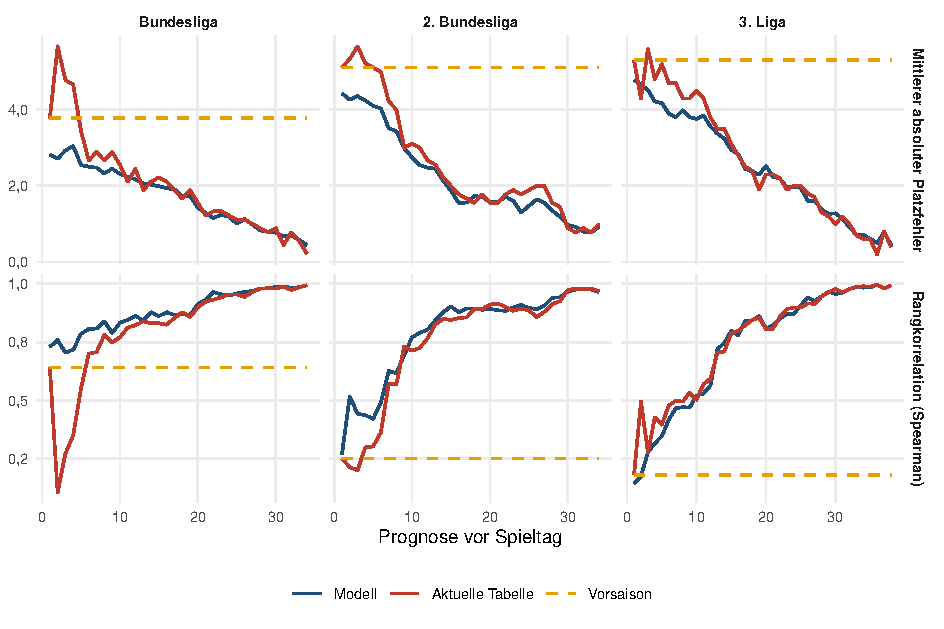
\includegraphics[width=\textwidth]{abbildungen/punktprognose_verlauf.pdf}
\caption{Rangmaße im Saisonverlauf. Oben: mittlerer absoluter Fehler des
Platzes (Modell: erwarteter Platz). Unten: Spearman-Korrelation mit der
Endtabelle.}\label{fig:punkt}
\end{figure}

\paragraph{Absicherung.} Die Stichtage einer Saison sind stark voneinander
abhängig, ein Test über sie wäre irreführend. Robuster ist der Vergleich je
Mannschaft. Wir mitteln die RPS-Differenz zur aktuellen Tabelle über alle
Stichtage und zählen, für wie viele Mannschaften das Modell besser war. In
der Bundesliga und der 2.~Bundesliga gilt das für je 17 von 18
Mannschaften, in der 3.~Liga für 17 von 20. Ein Vorzeichentest ergibt
$p < 0{,}003$ in jeder Liga. Gegenüber der Vorsaisontabelle sind es 17, 17
und 13 Mannschaften. Die 3.~Liga ist damit wieder die schwächste Liga für
das Modell ($p = 0{,}26$).

\begin{figure}[!htbp]
\centering
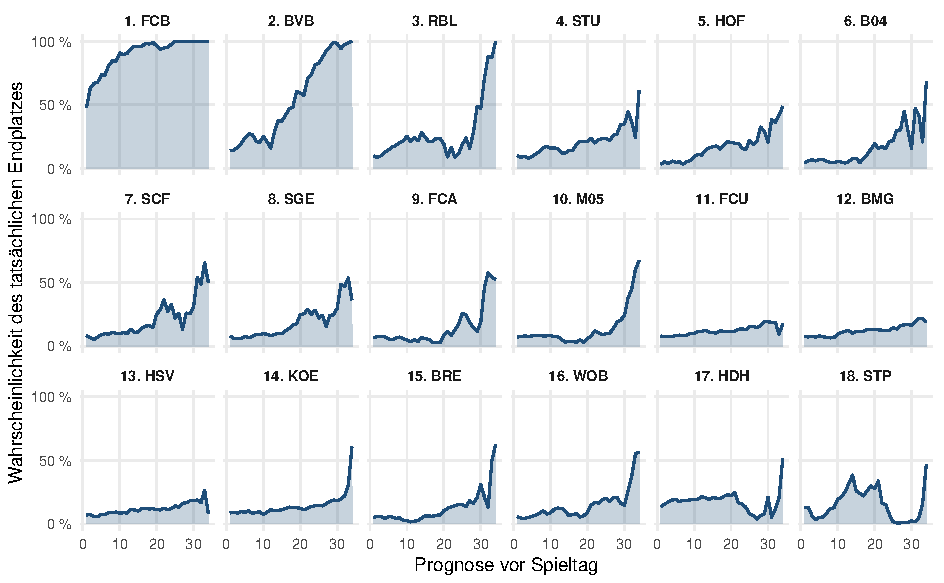
\includegraphics[width=\textwidth]{abbildungen/endplatz_verlauf_bl.pdf}
\caption{Bundesliga: prognostizierte Wahrscheinlichkeit für den
\emph{tatsächlichen} Endplatz, je Mannschaft vor jedem Spieltag. Das Format
übernimmt die Verlaufsgrafik aus dem Bericht von 2016.}\label{fig:endplatz}
\end{figure}

\abb{fig:endplatz} übernimmt die Verlaufsgrafik von 2016. Bayern lag vor dem
ersten Spieltag schon bei 48~Prozent für Platz~1 und ab dem 12.~Spieltag
dauerhaft über 90~Prozent. Dortmund lag ab dem 19.~Spieltag dauerhaft über 50~Prozent für
Platz~2. Im Mittelfeld blieb der genaue Platz wie 2016 bis kurz vor Schluss
offen. Die Mannschaften auf den Plätzen 9 bis 15 kamen erst in den letzten
Spieltagen über 30~Prozent für ihren späteren Platz. Auffällig ist
St.~Pauli: Zwischen dem 25. und 31.~Spieltag hielt das Modell Platz~18 für
fast ausgeschlossen, mit sechs Prognosen unter 2~Prozent. Die Gegenstücke für die 2.~Bundesliga und die
3.~Liga erzeugt das Auswertungsskript ebenfalls
(\datei{abbildungen/endplatz_verlauf_bl2.pdf}, \datei{..._l3.pdf}).

\subsection{Meisterschaft, Auf- und Abstieg}\label{sec:ereignisse}

Die Leser der Website interessieren sich weniger für den genauen Platz als
für die Spalten neben der Heatmap: Meister, Aufstieg, Abstieg.
\tab{tab:ereignisse} bewertet diese Ereignisse.

\begin{table}[!htbp]
\centering\footnotesize\setlength{\tabcolsep}{3.5pt}
\caption{Brier-Score für Platzgruppen, gemittelt über alle Mannschaften und
Stichtage, sowie Skill Score des Modells gegenüber der aktuellen Tabelle
und der Klimatologie (Anteil der Plätze). Spalte \enquote{Sp.\,1}: Brier vor
dem ersten Spieltag, Modell gegen Vorsaison.}\label{tab:ereignisse}
\begin{tabular}{@{}ll rrr rr r@{}}
\toprule
& & \multicolumn{3}{c}{Brier-Score} & \multicolumn{2}{c}{Skill gegenüber} & \\
\cmidrule(lr){3-5}\cmidrule(lr){6-7}
Liga & Ereignis & Modell & Tabelle & Klima & Tabelle & Klima & Sp.\,1 Mod.\,/\,Vors. \\
\midrule
BL  & Meister                 & 0,002 & 0,000 & 0,052 & $-\infty$ & 96\,\% & 0,020\,/\,0,000 \\
    & Champions League (1--4) & 0,069 & 0,088 & 0,173 & 21\,\% & 60\,\% & 0,115\,/\,0,222 \\
    & Relegation (16)         & 0,048 & 0,105 & 0,052 & 54\,\% &  9\,\% & 0,054\,/\,0,111 \\
    & Abstieg (17--18)        & 0,048 & 0,095 & 0,099 & 49\,\% & 51\,\% & 0,077\,/\,0,222 \\
\addlinespace
2.\,BL & Meister              & 0,040 & 0,046 & 0,052 & 13\,\% & 24\,\% & 0,059\,/\,0,111 \\
    & Direkter Aufstieg (1--2)& 0,063 & 0,095 & 0,099 & 33\,\% & 36\,\% & 0,105\,/\,0,222 \\
    & Aufstiegsrelegation (3) & 0,046 & 0,098 & 0,052 & 53\,\% & 12\,\% & 0,051\,/\,0,111 \\
    & Abstiegsrelegation (16) & 0,048 & 0,101 & 0,052 & 53\,\% &  9\,\% & 0,050\,/\,0,111 \\
    & Abstieg (17--18)        & 0,102 & 0,186 & 0,099 & 46\,\% & $-3$\,\% & 0,102\,/\,0,222 \\
\addlinespace
3.\,L & Meister               & 0,035 & 0,068 & 0,048 & 49\,\% & 26\,\% & 0,050\,/\,0,100 \\
    & Direkter Aufstieg (1--2)& 0,066 & 0,108 & 0,090 & 39\,\% & 27\,\% & 0,100\,/\,0,200 \\
    & Aufstiegsrelegation (3) & 0,043 & 0,095 & 0,048 & 55\,\% & 10\,\% & 0,047\,/\,0,100 \\
    & Abstieg (17--20)        & 0,047 & 0,055 & 0,160 & 15\,\% & 71\,\% & 0,144\,/\,0,200 \\
\bottomrule
\end{tabular}
\end{table}

Bis auf eine Ausnahme ist das Modell bei jedem Ereignis besser als die
aktuelle Tabelle, meist um 30 bis 55~Prozent. Die Ausnahme ist die
Bundesliga-Meisterschaft. Bayern stand ab dem zweiten Spieltag
ununterbrochen auf Platz~1 und war schon Vorjahresmeister. Beide naiven
Prognosen lagen damit die ganze Saison richtig und erreichen den Brier-Score
null, den keine Wahrscheinlichkeitsprognose schlagen kann. Das Modell kommt
mit 0,002 so nah heran, wie es mit ehrlicher Unsicherheit am Saisonanfang
möglich ist.

Gegenüber der Klimatologie fällt eine Zeile auf: der Abstieg aus der
2.~Bundesliga. Das Modell ist hier nicht besser als \enquote{jeder hat zwei
Achtzehntel}. Grund ist Fortuna Düsseldorf. Vor der Saison war Düsseldorf
für das Modell der drittstärkste Club der Liga, mit 3~Prozent
Abstiegswahrscheinlichkeit, und lag in keiner einzigen Prognose über
50~Prozent. Noch vor dem letzten Spieltag stand Düsseldorf auf Platz~15.
Am Ende hatten Braunschweig, Fürth und Düsseldorf je 37~Punkte, und
Düsseldorf war der schlechteste der drei.

\begin{table}[!htbp]
\centering\small
\caption{Ab welchem Spieltag lag die Prognose für den tatsächlichen Ausgang
\emph{dauerhaft} über 50 bzw.\ 90~Prozent? \enquote{--}: nie bis zum
letzten Stichtag. Auswahl.}\label{tab:abwann}
\begin{tabular}{@{}lll rrr@{}}
\toprule
Liga & Ereignis & Mannschaft & vor Sp.\,1 & $\ge 50\,\%$ ab & $\ge 90\,\%$ ab \\
\midrule
BL & Meister & Bayern München & 48\,\% & 2 & 12 \\
   & Champions League & Borussia Dortmund & 51\,\% & 3 & 19 \\
   & Champions League & RB Leipzig & 31\,\% & 28 & 31 \\
   & Champions League & VfB Stuttgart & 29\,\% & 34 & -- \\
   & Abstieg & 1.\,FC Heidenheim & 29\,\% & 15 & -- \\
   & Abstieg & FC St.\ Pauli & 25\,\% & 33 & -- \\
2.\,BL & Meister & FC Schalke 04 & 2\,\% & 30 & 32 \\
   & Abstieg & Preußen Münster & 22\,\% & 28 & 32 \\
   & Abstieg & Fortuna Düsseldorf & 3\,\% & -- & -- \\
3.\,L & Meister & VfL Osnabrück & 4\,\% & 29 & 35 \\
   & Direkter Aufstieg & Energie Cottbus & 6\,\% & 36 & -- \\
   & Abstieg & FC Schweinfurt 05 & 43\,\% & 2 & 11 \\
   & Abstieg & SSV Ulm 1846 & 3\,\% & 24 & 29 \\
\bottomrule
\end{tabular}
\end{table}

\tab{tab:abwann} zeigt, wie früh sich die Ausgänge abzeichneten. Klare
Fälle wie Bayern oder Schweinfurt erkannte das Modell früh. Die
Überraschungen der Saison, also Schalke, Osnabrück, Ulm und Düsseldorf,
lagen vor der Saison zwischen 2 und 4~Prozent. Das ist wenig, aber nicht
null. Bei 56~Mannschaften und mehreren Ereignissen je Liga sind einige
solche Ausgänge je Saison zu erwarten.

\subsection{Kalibrierung}\label{sec:kalibrierung}

\begin{figure}[!htbp]
\centering
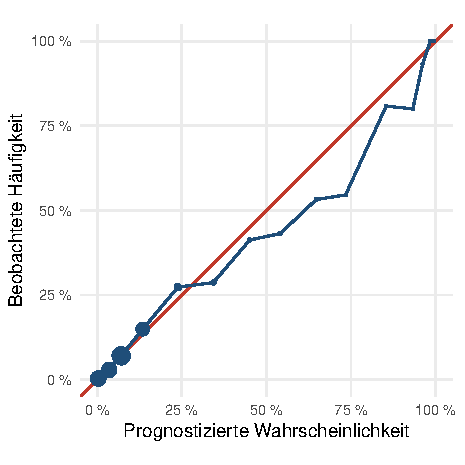
\includegraphics[width=0.48\textwidth]{abbildungen/kalibrierung_plaetze.pdf}\hfill
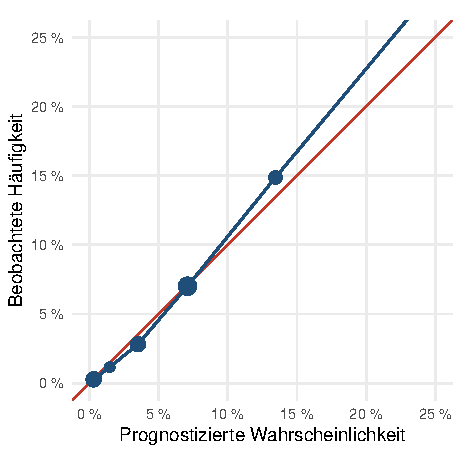
\includegraphics[width=0.48\textwidth]{abbildungen/kalibrierung_plaetze_zoom.pdf}
\caption{Kalibrierung der Platzwahrscheinlichkeiten, alle drei Ligen und
alle Stichtage. Rot: perfekte Kalibrierung. Punktgröße: Zahl der
Prognosen in der Klasse. Rechts: Ausschnitt bis 25~Prozent. Prognosen von
genau 0 und 100~Prozent sind ausgenommen.}\label{fig:kalib}
\end{figure}

\begin{table}[!htbp]
\centering\small
\caption{Kalibrierung nach Wahrscheinlichkeitsklassen (Auswahl) und
Extremprognosen.}\label{tab:kalib}
\begin{tabular}{@{}l rrrr@{}}
\toprule
Prognoseklasse & Prognosen & mittl.\ Prognose & eingetreten & erwartet \\
\midrule
0 bis 1\,\%   & \num{6076} &  0,3\,\% &  17 &  18,3 \\
1 bis 2\,\%   & \num{2320} &  1,5\,\% &  27 &  34,0 \\
2 bis 5\,\%   & \num{5929} &  3,5\,\% & 167 & 207,9 \\
5 bis 10\,\%  & \num{9223} &  7,1\,\% & 647 & 653,8 \\
10 bis 30\,\% & \num{5264} & 15,0\,\% & 884 & 792,1 \\
30 bis 50\,\% &        324 & 37,6\,\% & 105 & 121,6 \\
50 bis 80\,\% &        120 & 61,8\,\% &  59 &  74,2 \\
80 bis 100\,\%&         73 & 91,5\,\% &  63 &  67,2 \\
\midrule
genau 0\,\% (in keiner Simulation)   & \num{7888} & & 0 & \\
genau 100\,\% (in jeder Simulation)  & 15 & & 15 & \\
\bottomrule
\end{tabular}
\end{table}

\abb{fig:kalib} und \tab{tab:kalib} zeigen die Kalibrierung. Unter
10~Prozent, wo rund 80~Prozent aller Prognosen zwischen 0 und 100~Prozent
liegen, ist das Modell gut
kalibriert. Im Bereich 2 bis 5~Prozent liegt es leicht zu hoch, 167
Ereignisse statt der erwarteten 208. Die harten Ränder halten: \num{7888}
Prognosen von exakt null Prozent, kein einziger Treffer. Fünfzehnmal exakt
hundert Prozent, fünfzehn Treffer.

Darüber zeigt sich ein Muster, das dem Befund von 2016 entgegengesetzt ist.
Zwischen 10 und 30~Prozent trat mehr ein als prognostiziert (884 statt 792).
Zwischen 30 und 80~Prozent trat weniger ein (164 statt 196). Das Modell war
2025/26 also nicht zu zaghaft, sondern \emph{zu scharf}. Seine Favoriten
für einen Platz waren weniger sicher, als es angab, und die
Zweit- und Drittkandidaten kamen öfter zum Zug. Das passt zum logarithmischen
Score vor der Saison (Abschnitt~\ref{sec:vorsaison}) und zur Überschätzung der
Absteiger. Wegen der Abhängigkeit der Prognosen (siehe Kasten) ist die
Abweichung im Bereich 50 bis 80~Prozent für sich genommen kein harter
Beweis. Die Richtung ist aber über mehrere Klassen dieselbe.

\paragraph{Überraschungen unter 2~Prozent.} Von \num{8396} Prognosen mit
mehr als null und weniger als 2~Prozent trafen 44 ein, erwartet waren
52. 2016 waren es 12 von rund \num{2100}~\cite{30punkte2016}. Die Quote
ist mit 0,5 gegen 0,6~Prozent fast gleich. Die 44 verteilen sich auf neun
Mannschaften. Den größten Anteil haben zwei Fälle, in denen ein Platz im
Mittelfeld lange unwahrscheinlich aussah: Alemannia Aachen auf Platz~7 der
3.~Liga mit elf Prognosen, punktgleich mit Verl auf Platz~6, und Ulm auf
Platz~19, ebenfalls mit elf. Danach folgen Saarbrücken auf Platz~15
(sieben), St.~Pauli auf Platz~18 (sechs) und Düsseldorf auf Platz~17
(drei). Zweimal unter 2~Prozent lag Schalke als Meister, vor dem ersten und
dem dritten Spieltag.

\subsection{Einzelspiele}\label{sec:spiele}

Die Tabellenprognose ist nur so gut wie die Prognose der einzelnen Spiele.
Für jedes der 992~Spiele liegt die 1X2-Wahrscheinlichkeit vor, mit der ELO
unmittelbar vor dem Anpfiff aus dem chronologischen ELO-Walk.

\begin{table}[!htbp]
\centering\footnotesize\setlength{\tabcolsep}{3.5pt}
\caption{Einzelspiele: Gütemaße der 1X2-Prognose (Brier über drei Ausgänge,
RPS, Log-Loss) gegen die Klimatologie der Vorsaison und die
Gleichverteilung. Rechts: mittlere Prognose gegen beobachtete Quote.}\label{tab:spiele}
\begin{tabular}{@{}l r rrr rr r ccc@{}}
\toprule
& & \multicolumn{3}{c}{Brier} & \multicolumn{2}{c}{Log-Loss} & & \multicolumn{3}{c}{Prognose\,/\,beobachtet (\%)} \\
\cmidrule(lr){3-5}\cmidrule(lr){6-7}\cmidrule(l){9-11}
Liga & Spiele & Modell & Klima & Gleich & Modell & Klima & BSS & Heim & Remis & Ausw. \\
\midrule
Bundesliga    & 306 & \textbf{0,578} & 0,652 & 0,667 & \textbf{0,974} & 1,077 & 11,4\,\% & 41\,/\,44 & 24\,/\,25 & 35\,/\,32 \\
2. Bundesliga & 306 & \textbf{0,638} & 0,646 & 0,667 & \textbf{1,057} & 1,068 &  1,2\,\% & 40\,/\,46 & 26\,/\,24 & 34\,/\,30 \\
3. Liga       & 380 & \textbf{0,620} & 0,640 & 0,667 & \textbf{1,033} & 1,060 &  3,1\,\% & 40\,/\,46 & 26\,/\,23 & 34\,/\,31 \\
\midrule
Alle          & 992 & \textbf{0,613} & 0,646 & 0,667 & \textbf{1,022} & 1,068 &  5,1\,\% & 41\,/\,45 & 25\,/\,24 & 34\,/\,31 \\
\bottomrule
\end{tabular}
\end{table}

\tab{tab:spiele} zeigt: Das Modell schlägt die Klimatologie in jeder Liga.
In der Bundesliga ist der Vorsprung deutlich (Brier Skill Score 11~Prozent),
weil die Stärkeunterschiede dort groß sind. In der 2.~Bundesliga ist er mit
1~Prozent gering. Die Liga ist eng beieinander: Die Standardabweichung der Start-ELO
beträgt 63 Punkte gegen 129 in der Bundesliga. Viel mehr als die
Grundquoten ist da kaum zu holen. Der Favorit nach Modell gewann 54~Prozent der
Bundesligaspiele, 45~Prozent in der 2.~Bundesliga und 48~Prozent in der
3.~Liga.

\begin{figure}[!htbp]
\centering
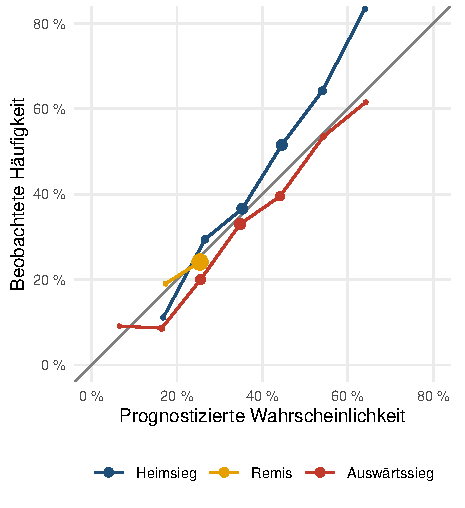
\includegraphics[width=0.46\textwidth]{abbildungen/kalibrierung_spiele.pdf}\hfill
\begin{minipage}[b]{0.5\textwidth}\small\captionsetup{justification=raggedright,singlelinecheck=false}
\captionof{figure}{Kalibrierung der 1X2-Wahrscheinlichkeiten, alle 992
Spiele, Klassen zu 10~Prozentpunkten (nur Klassen mit mindestens zehn
Prognosen). Die Heimsiege liegen über der Diagonalen, die Auswärtssiege
darunter.}\label{fig:spiele}
\vspace{1.5em}
\captionof{table}{Remisquote nach Stärkeunterschied $|\Delta|$ (mit
Heimvorteil 40).}\label{tab:remis}
\begin{tabular}{@{}lrrr@{}}
\toprule
$|\Delta|$ & Spiele & Prognose & beobachtet \\
\midrule
0--50     & 302 & 26,1\,\% & 26,2\,\% \\
50--100   & 254 & 25,9\,\% & 23,6\,\% \\
100--150  & 194 & 25,4\,\% & 25,3\,\% \\
150--200  & 103 & 24,7\,\% & 20,4\,\% \\
200--300  &  98 & 23,4\,\% & 22,4\,\% \\
über 300  &  41 & 19,2\,\% & 17,1\,\% \\
\bottomrule
\end{tabular}
\end{minipage}
\end{figure}

Die systematische Abweichung ist der Heimvorteil. Das Modell sagte im Mittel
41~Prozent Heimsiege voraus, es wurden 45. Bei den Auswärtssiegen lag es um
3~Prozentpunkte zu hoch, bei den Remis um gut 1~Punkt
(\abb{fig:spiele}). In der 2.~Bundesliga und der 3.~Liga sind es jeweils
6~Punkte Heimsiege zu wenig. In der Vorsaison 2024/25 lagen die
Heimsiegquoten bei 39, 41 und 45~Prozent, 2025/26 bei 44, 46 und
46~Prozent. Die Saison war also ungewöhnlich heimstark, und ein fester
Heimvorteil kann solche Schwankungen nicht abbilden. Bei den Remis bestätigt sich der
bekannte Befund: Das unabhängige Poisson-Modell ohne Korrekturterm nach
Dixon und Coles~\cite{dixoncoles1997} erzeugt eine Remisquote, die
mit wachsendem Stärkeunterschied nur langsam fällt (\tab{tab:remis}). Bei
gleich starken Teams trifft es die Quote genau, bei mittleren Unterschieden
liegt es etwas zu hoch.

\subsection{Robustheit: Heimvorteil 65 statt 40}\label{sec:robust}

Bis September 2026 rechnete das Modell produktiv mit einem Heimvorteil von
65 ELO-Punkten. Die damals veröffentlichten Prognosen entsprechen also nicht
genau der Rückrechnung oben. Wir haben die ganze Auswertung mit $H = 65$
wiederholt (Verzeichnis \datei{daten_ha65/}). Die Platzprognosen ändern sich
praktisch nicht. Der RPS im Saisonmittel weicht in keiner Liga um mehr als
0,0003 ab, und alle Aussagen der Abschnitte~\ref{sec:vorsaison}
bis~\ref{sec:kalibrierung} gelten unverändert. Bei den Einzelspielen
schneidet $H = 65$ in dieser heimstarken Saison minimal besser ab (Brier
0,610 statt 0,613, mittlere Heimsiegprognose 43 statt 41~Prozent). Für die
Tabelle spielt der Heimvorteil kaum eine Rolle, weil in einer Doppelrunde
jede Mannschaft gleich oft zu Hause spielt.

\section{Diskussion}\label{sec:diskussion}

\paragraph{Was das Modell kann.} Über eine Saison gesehen ist das Modell eine
deutlich bessere Wahrscheinlichkeitsprognose als die naheliegenden
Alternativen. Am größten ist sein Wert in der ersten Saisonhälfte. Dort ist
die Tabelle noch stark vom Zufall geprägt, und dort fragen die Leser am
meisten danach, was der Stand bedeutet. Die harten Aussagen stimmen
ausnahmslos: Was das Modell in \num{10000} Durchläufen nie sah, trat nie ein,
und was es immer sah, trat immer ein. Für eine öffentliche Prognose ist das
die wichtigste Eigenschaft.

\paragraph{Was es nicht kann.} Vor der Saison weiß das Modell in der
2.~Bundesliga und der 3.~Liga kaum mehr als eine Gleichverteilung, und
manchmal ist es sich dabei zu sicher. Das hat zwei Ursachen, die man im Code
angehen kann:
\begin{enumerate}
  \item \textbf{Übertrag ohne Rückführung.} Absteiger bringen ihre ELO aus
        der höheren Liga mit und werden in der neuen Liga systematisch
        überschätzt. Mit vier Fällen ist das noch kein belastbarer Befund,
        die Richtung ist aber eindeutig, und sie deckt sich mit der
        Erfahrung aus anderen ELO-Systemen. Viele davon ziehen zum Saisonwechsel
        jeden Wert ein Stück zum Mittel zurück, verbreitet ist etwa ein
        Drittel.
        Ein solcher Abschlag, für Absteiger womöglich stärker, ist der
        naheliegende nächste Versuch. Er lässt sich an den Saisons 2019 bis
        2024 aus dem Fixture-Cache prüfen, ohne die Saison 2025/26 zur
        Eichung zu benutzen.
  \item \textbf{Zu wenig Streuung in der Stärke.} Das Modell kennt nur die
        Unsicherheit der Spielausgänge, nicht die Unsicherheit über die
        Stärke selbst. Zwar wird die ELO innerhalb jeder Simulation
        fortgeschrieben, das verbreitert die Verteilung aber nur wenig.
        Die zu scharfe Kalibrierung zwischen 30 und 80~Prozent passt dazu.
        Ein Ausweg wäre, je Iteration die Start-ELO jeder Mannschaft mit
        einem Zufallsaufschlag zu ziehen. Dessen Größe ließe sich wieder an
        Vorsaisons eichen.
\end{enumerate}
Hinzu kommt der Heimvorteil, der von Saison zu Saison schwankt. Ein fester
Wert wird immer einmal zu hoch und einmal zu niedrig liegen. Für die
Tabellenprognose ist das, wie gezeigt, fast bedeutungslos, für die 1X2-Anzeige
nicht.

\paragraph{Grenzen dieser Auswertung.} Eine Saison ist eine Stichprobe von
eins. Die Überraschungen von 2025/26 wie Schalke, Düsseldorf und Ulm prägen
die Zahlen stark, und eine andere Saison kann anders aussehen. Ein
Vergleich mit Wettquoten, dem eigentlich strengen Maßstab, fehlt mangels
Daten. Die Prognosen sind nachgerechnet und nicht archiviert. Sie folgen
aber demselben Code und denselben Startwerten. Die Abweichung durch den
damaligen Heimvorteil ist in Abschnitt~\ref{sec:robust} beziffert. Künftig
sollte der Scheduler die Matrix jedes Stichtags ablegen, damit die nächste
Bilanz die tatsächlich veröffentlichten Zahlen bewerten kann.

\section{Fazit}

\begin{merke}[Die Saison 2025/26 in fünf Sätzen]
\begin{enumerate}[leftmargin=*,itemsep=1pt]
  \item Im Saisonverlauf schlägt das Modell die aktuelle Tabelle in allen
        drei Ligen klar: RPS 35 bis 44~Prozent besser, an 104 von
        106~Stichtagen vorn.
  \item Als reine Rangfolge ist der Vorsprung klein. In der zweiten
        Saisonhälfte ist die Tabelle gleichauf, in der 3.~Liga sogar knapp
        vorn.
  \item Vor der Saison schlägt das Modell die Vorsaisontabelle in jeder Liga.
        In der 2.~Bundesliga und der 3.~Liga ist es aber kaum besser als
        der blinde Zufall. Absteiger werden überschätzt.
  \item Unter 10~Prozent ist das Modell gut kalibriert, und die Ränder 0 und
        100~Prozent halten ausnahmslos. Dazwischen ist es etwas zu scharf.
  \item Die Einzelspiele schlagen die Grundquoten. Den Heimvorteil der
        Saison 2025/26 unterschätzt das Modell um rund fünf Prozentpunkte.
\end{enumerate}
\end{merke}

Das Urteil von 2016 lässt sich also übernehmen und präzisieren: nicht allzu
schlecht und deutlich besser als ein Blick auf die Tabelle. Die
Verbesserungsmöglichkeiten liegen beim Saisonstart.

\appendix
\section{Vorsaisonprognosen je Mannschaft}\label{anh:teams}

Sortiert nach dem Endplatz. \enquote{Vorsaison}: Liga und Platz 2024/25 (RL:
Regionalliga-Meister). \enquote{E[Platz]} und \enquote{Rang}: erwarteter Platz
und Rangfolge des Modells vor Spieltag~1. \enquote{Naiv}: Platz nach der
Vorsaisonregel aus Abschnitt~\ref{sec:aufbau}.

\newcommand{\teamtab}[2]{%
\begin{table}[!htbp]\centering\small
\caption{#1}
\begin{tabular}{@{}rl l r r r r r@{}}
\toprule
Ende & Mannschaft & Vorsaison & Start-ELO & E[Platz] & Rang & Naiv & Punkte \\
\midrule
\csname @@input\endcsname tabellen/#2.tex 
\bottomrule
\end{tabular}
\end{table}}
\teamtab{Bundesliga 2025/26}{vorsaison_bl}
\teamtab{2.~Bundesliga 2025/26}{vorsaison_bl2}
\teamtab{3.~Liga 2025/26}{vorsaison_l3}

\clearpage
\section{Reproduktion}\label{anh:repro}

Alle Zahlen und Abbildungen entstehen aus zwei Skripten. Vorausgesetzt sind
ein laufender Rust-Server und der Fixture-Cache \datei{data/fixture_cache/}
für die Saisons 2024 und 2025. Ohne Cache werden die Spiele über die API
geholt, dann ist \code{RAPIDAPI\_KEY} nötig.
\begin{verbatim}
cd league-simulator-rust && cargo build --release
./target/release/league-simulator-rust &      # Port 8080
cd ..
D=docs/reports/2026-10-11-prognoseguete-2025-26
Rscript scripts/evaluate_forecast_quality.R 2025 $D/daten
Rscript scripts/evaluate_forecast_quality.R 2025 $D/daten_ha65 65
Rscript scripts/analyze_forecast_quality.R  $D
cd $D && latexmk prognoseguete-2025-26.tex
\end{verbatim}
Das erste Skript schreibt je Liga und Stichtag die Platzmatrix
(\datei{positions.csv}), die Tabellenstände (\datei{snapshots.csv}), die
1X2-Prognosen aller Spiele (\datei{matches.csv}) und die Mannschaftsdaten
(\datei{teams.csv}). Das zweite berechnet daraus die Gütemaße
(\datei{ergebnisse/}), die Abbildungen und die Anhangtabellen. Wegen der
Monte-Carlo-Ziehung weicht ein neuer Lauf in der dritten Nachkommastelle
ab. An den Aussagen ändert das nichts.

\begin{thebibliography}{9}\small
\bibitem{30punkte2016} 30 Punkte: \emph{Qualität der Prognosen: Bundesliga.}
  15.~Mai 2016.
  \url{https://30punkte.wpcomstaging.com/2016/05/15/qualitaet-der-prognosen-bundesliga/}
\bibitem{brier1950} G.\,W. Brier: Verification of forecasts expressed in
  terms of probability. \emph{Monthly Weather Review} 78 (1950), 1--3.
\bibitem{epstein1969} E.\,S. Epstein: A scoring system for probability
  forecasts of ranked categories. \emph{Journal of Applied Meteorology} 8
  (1969), 985--987.
\bibitem{gneiting2007} T. Gneiting, A.\,E. Raftery: Strictly proper scoring
  rules, prediction, and estimation. \emph{Journal of the American
  Statistical Association} 102 (2007), 359--378.
\bibitem{constantinou2012} A.\,C. Constantinou, N.\,E. Fenton: Solving the
  problem of inadequate scoring rules for assessing probabilistic football
  forecast models. \emph{Journal of Quantitative Analysis in Sports} 8
  (2012).
\bibitem{hvattum2010} L.\,M. Hvattum, H. Arntzen: Using ELO ratings for
  match result prediction in association football. \emph{International
  Journal of Forecasting} 26 (2010), 460--470.
\bibitem{dixoncoles1997} M.\,J. Dixon, S.\,G. Coles: Modelling association
  football scores and inefficiencies in the football betting market.
  \emph{Applied Statistics} 46 (1997), 265--280.
\end{thebibliography}

\end{document}
